


\begin{frame}[fragile]{PETSc Vectors}

 \begin{block}{Parallel Vector Layout}
   \begin{center}
     \includegraphics[width=0.75\textwidth]{figures/vectors} \\[2em]
   \end{center}
\begin{lstlisting}
  VecCreate(PETSC_COMM_WORLD, &x);
  VecSetSizes(x, PETSC_DECIDE, N);
  VecSetFromOptions(x);
\end{lstlisting}
  \vspace*{2.3cm}
 \end{block}

\end{frame}

\begin{frame}[fragile]{PETSc Vectors}

 \begin{block}{Vector Gather and Scatter}
   \begin{center}
     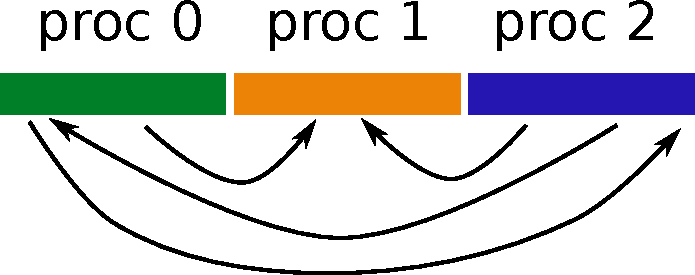
\includegraphics[width=0.75\textwidth]{figures/vectors-scatter} \\[1em]
\begin{lstlisting}
  // y[iy[i]] = x[ix[i]]
  VecScatterCreate(...);
  VecScatterBegin(...);
  VecScatterEnd(...);
\end{lstlisting}
   \end{center}
 \end{block}

\end{frame}

%%%%%%%%%% 


\begin{frame}[fragile]{PETSc Vectors}

 \begin{block}{Vector Reductions}
   \begin{center}
     \includegraphics[width=0.75\textwidth]{figures/vectors-reduce} \\[1.2em]
\begin{lstlisting}
  VecNorm(...);
  VecDot(...);
  VecMax(...);
  ...
\end{lstlisting}
   \end{center}
 \end{block}

\end{frame}


%%%%%%%%%% 

\begin{frame}[fragile]{PETSc Vectors}

 \begin{block}{Local (Sequential) Operations}
  \begin{itemize}
   \item Executed by an arbitrary subset of MPI ranks
   \item Usually involve \lstinline|VecGetArray()/VecRestoreArray()|
  \end{itemize}
 \end{block}

 %\pause
 
 \begin{block}{Collective Operations}
  \begin{itemize}
   \item Must be executed by all processes in the MPI communicator
   \item Involve MPI operations (scatter, gather, reduce, etc.)
  \end{itemize}
 \end{block}

\end{frame}
